\begin{apendicesenv}

    \chapter{Software metrics}
    \label{appe:A}
    
    \section{List of class-level software metrics}
    
    Table \ref{tab:classLevelMetricsList} show the entire list of class-level metrics\footnotemark ~used to collect independent variables.
    \footnotetext{https://scitools.com/feature/metrics/}
    
\begin{center}
\footnotesize
\begin{longtabu} to \linewidth {@{}lX@{}}
\toprule
\textbf{metric name} & \textbf{description} \\ 
\midrule
\endhead
Average Cyclomatic Complexity & Average cyclomatic complexity for all nested functions or methods. \\
Avg Number of Blank Lines & Average number of blank lines for all nested functions or methods. \\
Avg Number of Lines & Average number of lines for all nested functions or methods. \\
Avg Number of Lines of Code & Average number of lines containing source code for all nested functions or methods. \\
Avg Number of Lines with Comments & Average number of lines containing comment for all nested functions or methods. \\
Base Classes & Number of immediate base classes \\
Class Methods & Number of class methods \\
Class Variables & Number of class variables \\
Comment to Code Ratio & Ratio of number of comment lines to number of code lines. \\
Coupling Between Objects & The Coupling Between Object Classes (CBO) measure for a class is a count of the number of other classes to which it is coupled. Class A is coupled to class B if class A uses a type, data, or member from class B. Any number of couplings to a given class counts as 1 towards the metric total. \\
Declarative Statements & Number of declarative statements \\
Depth of Inheritance Tree (DIT) & The depth of a class within the inheritance hierarchy is the maximum number of nodes from the class node to the root of the inheritance tree. The root node has a DIT of 0. The deeper within the hierarchy, the more methods the class can inherit, increasing its complexity. \\
Executable Lines of Code & Number of lines containing executable source code. \\
Instance methods & Number of instance methods \\
Instance Variables & Number of instance variables - variables defined in a class that are only accessable through an object of that class \\
Lines with Comments & Number of lines containing comment.~ \\
Lines with Source Code & The number of lines that contain source code.~ \\
Local Default Visibility Methods & Number of local default visibility methods \\
Max Cyclomatic Complexity & Maximum cyclomatic complexity of all nested functions or methods. \\
Maximum nesting level & Maximum nesting level of control constructs (if, while, for, switch, etc.) in the function. \\
Number of blank lines & Number of blank lines \\
Number of Children & Number of immediate subclasses. (i.e. the number of classes one level down the inheritance tree from this class). \\
Number of declarative Lines of Code & Number of lines containing declarative source code. Note that a line can be declarative and executable. Example: int i = 0; \\
Number of Local Methods (WMC) & Number of local (not inherited) methods. \\
Number of Methods & Number of methods, including inherited ones. \\
Physical lines & Number of physical lines. \\
Percent Lack of Cohesion in Methods & 100\% minus average cohesion for class data members. Calculates what percentage of class methods use a given class instance variable. A lower percentage means higher cohesion between class data and methods. \\
Private Methods & Number of local (not inherited) private methods. \\
Protected Methods & Number of local protected methods. \\
Public Methods & Number of public methods. Only counts local (not inherited) methods. \\
Statements & Number of declarative plus executable statements. \\
Sum of Cyclomatic Complexity & Sum of cyclomatic complexity of all nested functions or methods. \\
\bottomrule
\caption{List of class-level metrics}
\label{tab:classLevelMetricsList}
\end{longtabu}
\end{center}

\section{List of method-level software metrics}
    
Table \ref{tab:methodLevelMetricsList} show the entire list of method-level metrics\footnotemark ~used to collect independent variables.
\footnotetext{https://scitools.com/feature/metrics/}
    
\begin{center}
\footnotesize
\begin{longtabu} to \linewidth {@{}lX@{}}
\toprule
\textbf{metric name} & \textbf{description} \\ 
\midrule
\endhead
Number of inputs & The number of inputs a function uses plus the number of unique subprograms calling the function. Inputs include parameters and global variables that are used in the function. \\
Number of blank lines & Number of blank lines. \\
Source Lines of Code & The number of lines that contain source code. A line can contain source and a comment and thus count towards multiple metrics. \\
Number of declarative lines of Code & Number of lines containing declarative source code. A line can be declarative and executable. Example: int i =0; \\
Executable Lines of Code & Number of lines containing executable source code. \\
Lines with Comments & Number of lines containing comment. \\
Number of outputs (FANOUT) & The number of outputs that are SET. This can be parameters or global variables.~ \\
Paths & Number of unique paths though a body of code, not counting abnormal exits or gotos. \\
Statements & Number of declarative plus executable statements. \\
Declarative Statements & Number of declarative statements. \\
Executable Statements & Number of executable statements. \\
Cyclomatic Complexity & The cyclomatic complexity of any structured program with only one entrance point and one exit point is equal to the number of decision points contained in that program plus one. It counts the keywords for decision points (FOR, WHILE, etc) and then adds 1. \\
Maximum nesting level & Maximum nesting level of control constructs (if, while, for, switch, etc.) in the function. \\
Comment to Code Ratio & Ratio of number of comment lines to number of code lines. Some lines are both code and comment, so this could easily yield percentages higher than 100.\\
\bottomrule
\caption{List of method-level metrics}
\label{tab:methodLevelMetricsList}
\end{longtabu}
\end{center}

    \newpage

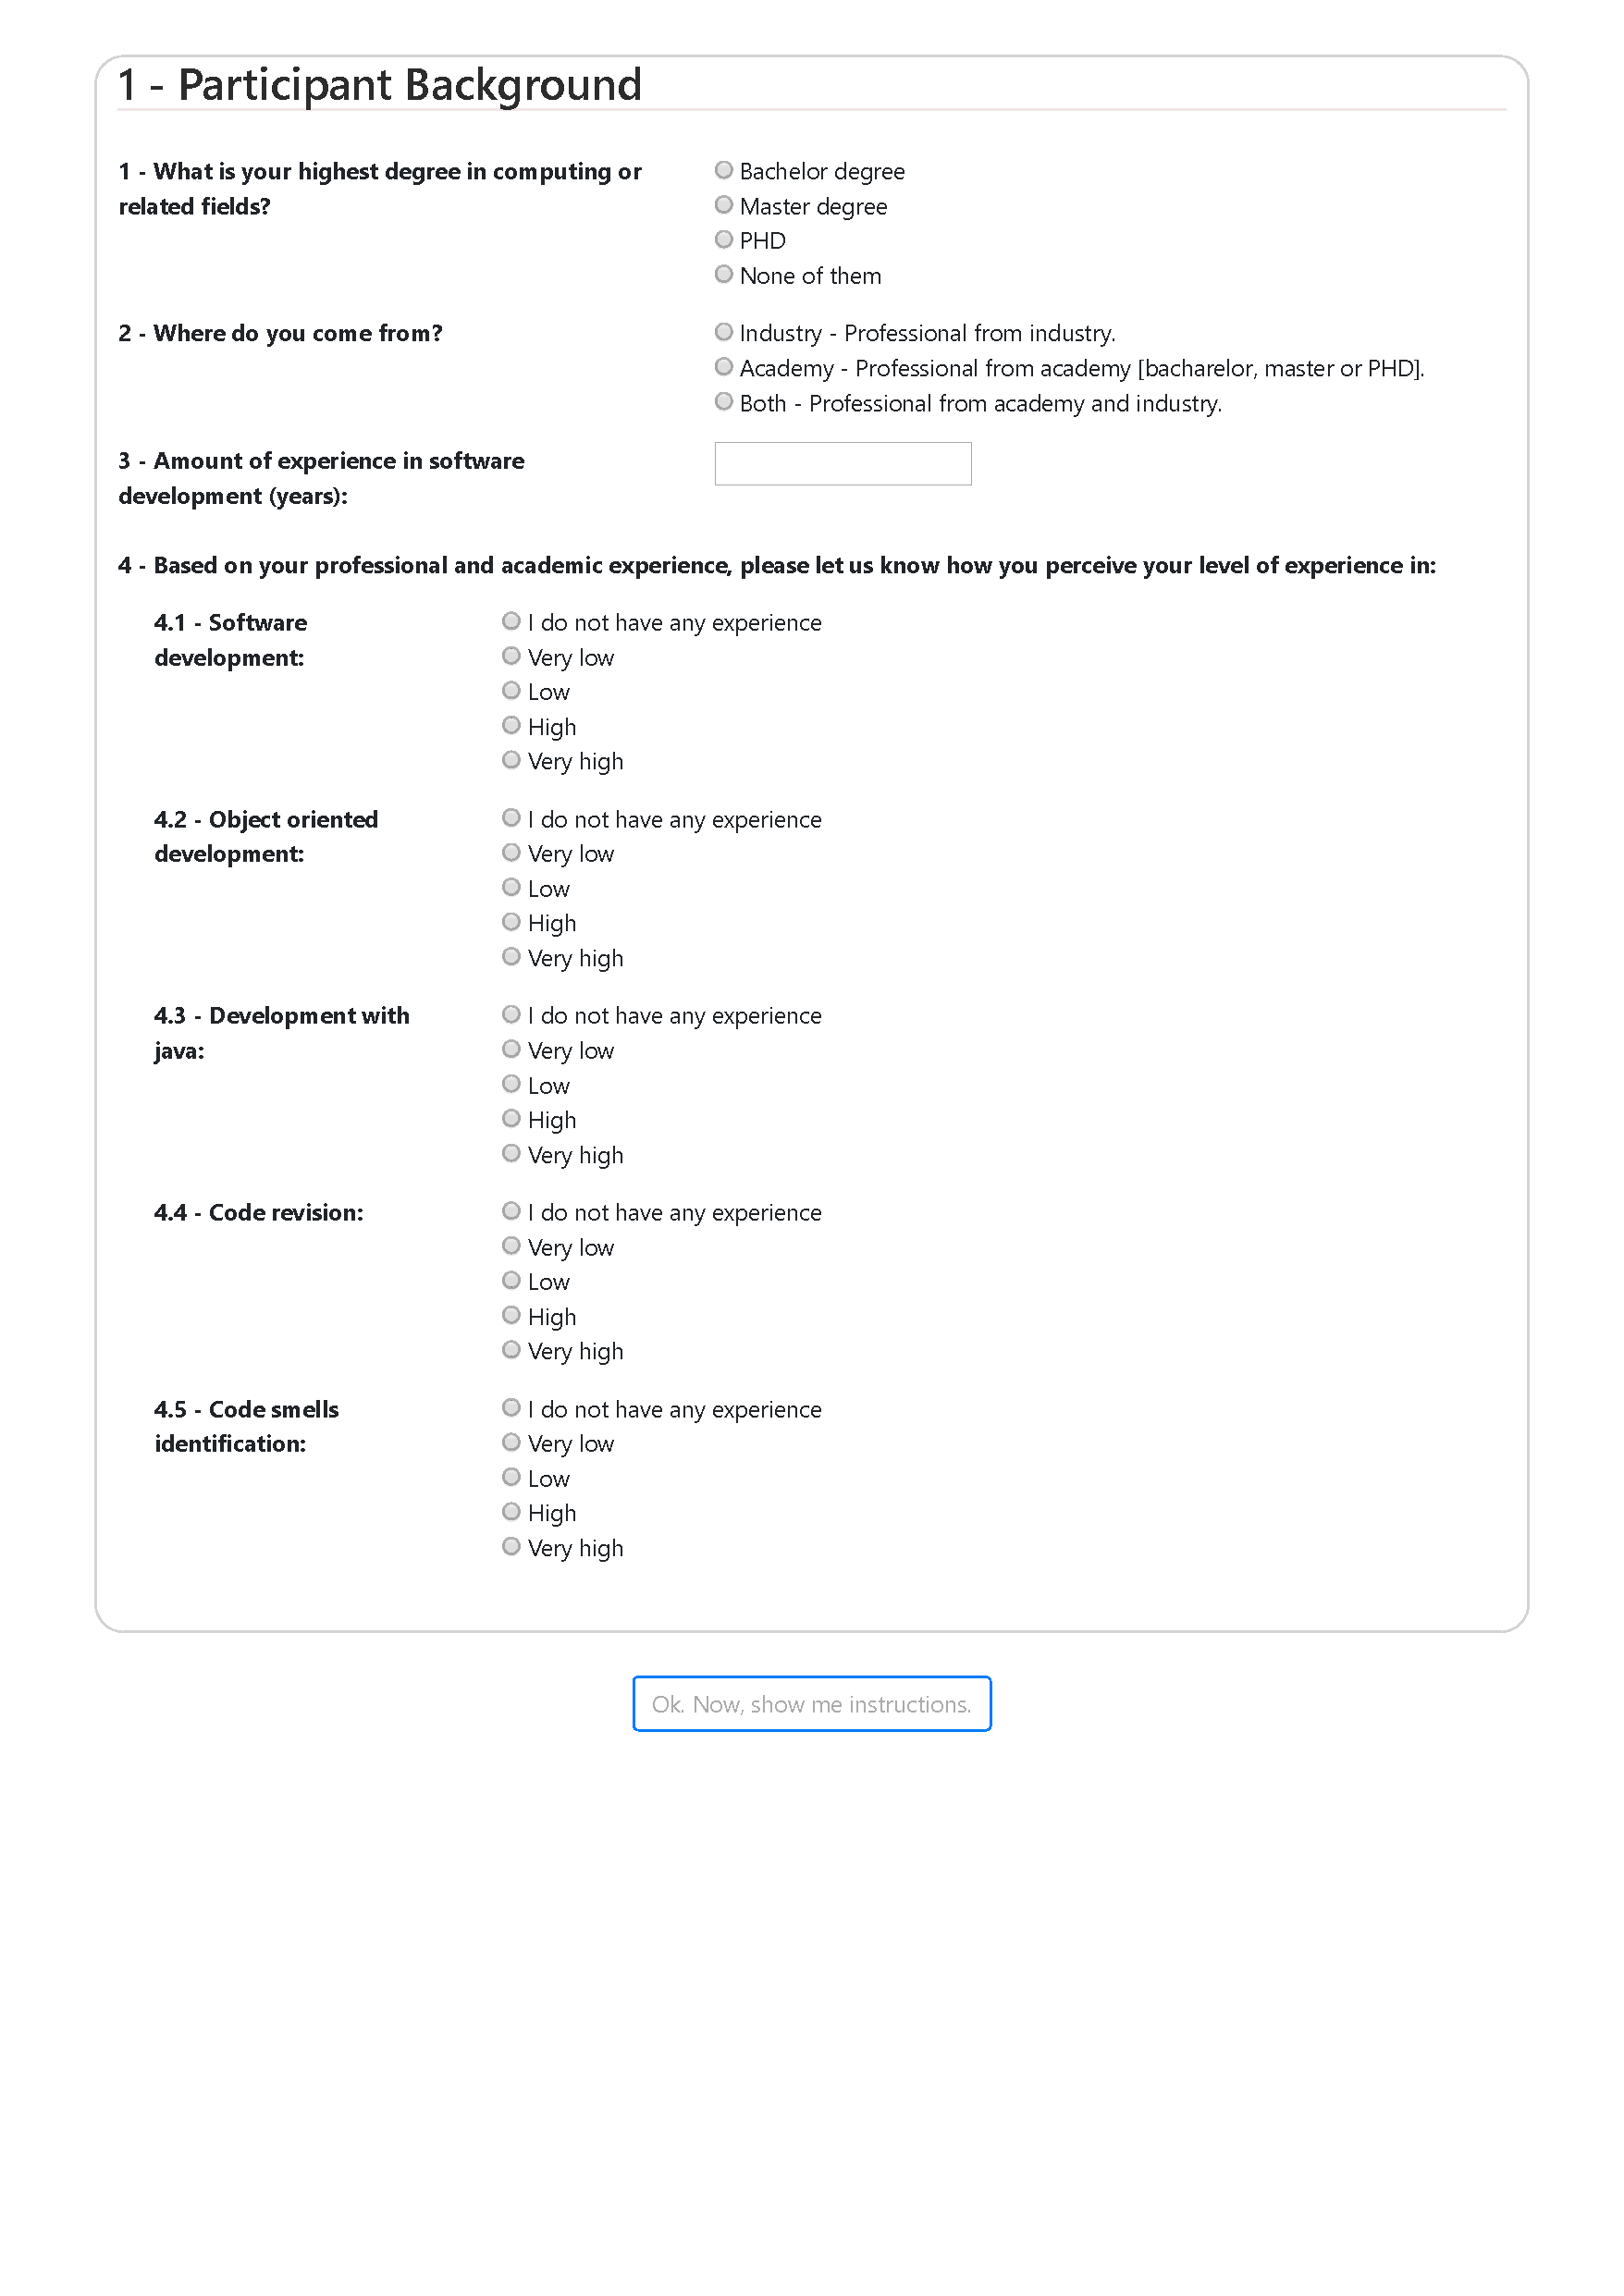
\includepdf[pages=-,scale=0.8,pagecommand={\chapter{Participant background questionnaire}\label{appe:B}},linktodoc=true]{participantBackground.pdf}


\end{apendicesenv}





